\documentclass[10pt,a4paper,ngerman]{scrartcl}
\usepackage[utf8]{inputenc}
\usepackage[british]{babel}
\usepackage[T1]{fontenc}
\usepackage{amsmath}
\usepackage{amsfonts}
\usepackage{amssymb}
\usepackage{makeidx}
\usepackage{graphicx}
\usepackage{epstopdf}
\usepackage[onehalfspacing]{setspace}
\usepackage{array}
\usepackage{upgreek}
\usepackage{float}
\usepackage{csquotes}
\usepackage{chemformula}
\usepackage{chemgreek}
\usepackage{chemmacros}
\chemsetup{modules=all}
\usepackage{tikz}
\usepackage{siunitx}
\sisetup{locale = DE,per-mode = symbol}
\usepackage{esvect}
\usepackage{geometry}
\usepackage{pdfpages}
\usepackage[font=small]{caption}
%\usepackage[version=4]{mhchem}
\usepackage[backend=biber, style=chem-angew]{biblatex}
\addbibresource{Rheo.bib}
\usepackage{tabularx, booktabs, multirow}
\usepackage[pdfborder={0 0 0}]{hyperref}
\usepackage{cleveref}
\newcommand{\crefrangeconjunction}{--}
\crefrangelabelformat{equation}{#3#1#4--#5#2#6}
\usepackage{scrlayer-scrpage}%Header für die KOMA-script -Klasse
%\usepackage{hyperref}
\usepackage{pgfplots}
\usepackage{textgreek}


\newcommand{\tildenu}{{\fontencoding{LGR}\selectfont\accperispomeni\textnu}}
\captionsetup{format=plain}
\chemsetup[phases]{pos=sub}
\chemsetup[redox]{pos=top}
\chemsetup[redox]{align=center}
%\chemsetup[redox]{explicit-sign=true}
%\chemsetup[redox]{roman=false}
\newcommand{\celsius}{^{\circ}\mathrm{C}}
\parindent0pt
\sloppy
\DeclareChemPhase{\s}{s}
\DeclareChemPhase{\l}{l}
\DeclareChemPhase{\g}{g}
\renewcaptionname{ngerman}{\figurename}{Abb.}
\renewcaptionname{ngerman}{\tablename}{Tab.}
\geometry{bottom=100pt} \geometry{top=80pt}
\newcommand{\m}{\mathrm{m}}
\newcommand{\K}{\mathrm{K}}
\newcommand{\J}{\mathrm{J}}
\newcommand{\gr}{\mathrm{g}}
\newcommand{\kg}{\mathrm{kg}}
\newcommand{\mol}{\mathrm{mol}}
\newcommand{\Pa}{\mathrm{Pa}}
\newcommand{\ad}{\mathrm{ad}}
\newcommand{\de}{\mathrm{de}}
\newcommand{\gmol}{\mathrm{\frac{g}{mol}}}
\newcommand{\JKmol}{\mathrm{\frac{J}{K \cdot mol}}}
\newcommand{\kgmss}{\mathrm{\frac{kg}{m \cdot s^2}}}
\newcommand{\loge}{\mathrm{ln}}

\begin{document}
\begin{titlepage}
	\vspace*{2,5cm}
	\begin{center}
		\begin{LARGE}
			\textbf{Polymeric Chemistry}\\
			\textbf{Rheology}\\
		\end{LARGE}
		\vspace{1cm}
		\textbf{Universität Stuttgart}\\
		\vspace*{1,5cm}
		\begin{tabular}{lp{7,5cm}l}
			Author 1:     & Laurens Viehoff\\
            Author 2:     & Felix Roth\\   
			E-Mail 1:     & st183688@stud.uni-stuttgart.de\\
            E-Mail 2:     & st188157@stud.uni-stuttgart.de  \\
			Student-ID 1: & 3676761   \\ 
            Student-ID 2: & 3711192 \\ \\
			Assistent:    & Semi Kim   \\ \\ 
		\end{tabular}
	\end{center}
    
\end{titlepage}
\thispagestyle{empty}
\renewcommand{\thepage}{\arabic{page}}
\newpage
\tableofcontents
\setcounter{page}{1}
\renewcommand{\thepage}{\arabic{page}}
\newpage

\section{Theory}
		In rheology, the flow behaviour of a substance under different forces is studied. This behaviour can be determined using rotational or oscillatory measurements.
	
	\subsection{Basic concepts}
		To measure rheological properties, the sample is placed between two plates, the upper one of which is capable of moving. When this plate is set in motion, the 
		sample experiences a force and moves along with it, but exhibits a velocity gradient from the lower to the upper plate. A visual representation of this is shown 
		in Figure \ref{RheoModell}.

		\begin{figure}[H]
            \centering
            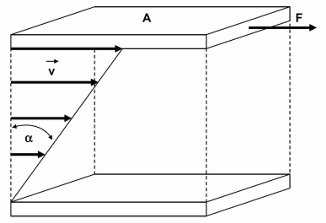
\includegraphics[scale = 0.7]{Bilder/RheoModell.png}
            \caption{The diagram shows two plates with an area $A$, the upper one of which exerts a force $F$ on the specimen, causing it to experience a velocity gradient $\vec{v}$ and to move through an angle $\alpha$. \cite{polyskript}}
            \label{RheoModell}
        \end{figure}

		Key parameters that can be detected or specified in this context include deformation $\gamma$, deformation rate $\dot{gamma}$, shear stress $\tau$ and 
		steady-state shear viscosity $\eta$. These parameters are defined by Equations (\labelcref{gamma,gammadot,tau,eta}).

		\begin{align}
			\label{gamma}
			&\text{Deformation:}  &\gamma &\equiv \frac{dx}{dy} = \tan \alpha  \\
			\label{gammadot}
			&\text{Deformation rate:}  &\dot{\gamma} &\equiv \frac{d\gamma}{dt} \\
			\label{tau}
			&\text{Shear stress:}  &\tau &= \frac{F}{A} = \eta \cdot \dot{\gamma}  \\
			\label{eta}
			&\text{Steady-state shear viscosity:}  &\eta &= \frac{\tau}{\dot{\gamma}}
		\end{align}

		$x$ and $y$ represent the coordinate axes, with $x$ pointing in the direction of the force $F$. \cite{polyskript}\\
		If a strain rate is specified and the shear stress is thereby detected, the viscosity can also be determined, allowing these parameters to be investigated as 
		a function of the strain rate. Three types of curve behaviour can be detected for the shear stress or viscosity. The parameters may follow a linear trend or 
		deviate from it. If the parameters deviate, they may become either larger or smaller at higher deformation rates. If a sample exhibits a linear relationship, 
		it is referred to as a Newtonian fluid. If the parameters increase at higher deformation rates, it is referred to as a non-Newtonian shear-thickening fluid; 
		conversely, if they decrease, it is referred to as a non-Newtonian shear-thinning fluid.
		For example, Figure \ref{honey} shows the experimental behaviour of a Newtonian fluid, Figure \ref{14PVP} that of a shear-thinning fluid, and Figure \ref{starch} 
		that of a shear-thickening fluid. \cite{polyskript}

	\subsection{Behaviour of matter}
		
		\subsubsection{Elastic}
			The elastic behaviour of a polymer can be compared to that of a rubber band or a spring. When a force is applied, causing deformation or shear stress, 
			the polymer responds by undergoing shear or deformation, and returns to its original state once the force is removed. \cite{polyskript}
		\subsubsection{Viscous}
			In the case of viscous behaviour, the material deforms continuously when a force is applied and retains its deformation once the force is removed. \cite{polyskript}
		\subsubsection{Plastic}
			In the case of plastic behaviour, the material only deforms once a certain stress level is reached; prior to this, it behaves either elastically or shows 
			no deformation. \cite{polyskript}
		\subsubsection{viscoelastic}
			Most materials exhibit viscoelastic behaviour, which describes a combination of elastic and viscous behaviour. When a stress is applied, the material will 
			deform elastically and then continue to deform under further shear stress. If this stress is removed, the deformation is partially reversed, but a slight 
			deformation remains. This residual deformation depends on whether the material exhibits more elastic or viscous behaviour. \\
			
			
	
	\subsection{Measurement methods}
		As mentioned at the start, in rheological measurements the sample is placed between two plates and moved through the upper plate. However, in a plate-plate 
		geometry, the rate of deformation of the material depends on the radius. For this reason, the upper plate is often replaced by a slightly conical plate. This 
		conical plate can then be rotated or oscillated. During rotation, the conical plate can be rotated at different speeds, with either the strain rate or the 
		stress being applied. This allows the viscosity, strain rate and shear stress to be determined. During oscillation, the stress or strain is again applied, and the 
		other quantity is thereby determined Furthermore, the cone plate is oscillated only up to a certain deflection and at a specific frequency. This is used to 
		measure the complex viscosity η, the viscoelasticity and, at the same time, the extent to which the material is more viscous or elastic. The entire process is 
		determined by varying the deflection and subsequently selecting the frequency, and follows the equations below.\\
	
	\subsection{}
\section{Results}

	\subsection{Rotational measurements}

		After analyzing the different graphs it can be stated that honey has the typicall linear progression wich speaks for a newtonian fluid.
		By analyzing Graph \ref{honey} in the area from $10^{-1}$-$10^{0}$ of the deformation velocity a non linear part can be observed.
		However, this does not mean that honey is a non-Newtonian fluid, but rather that it takes a certain amount of time before measurement accuracy can be guaranteed.
		This comes from the first "loosening" of the molecules, because these can be intertwinded or stuck in each other.
		This can also be applied on the other measurements.

		

		\begin{figure}[H]
			\centering
			
\includegraphics[scale = 0.5]{Bilder/Honey.png}
			\caption{The graph shows the measurements of honey. 
			On the left y-axis the shear stress and on the right y-axis the velocity is plotted, both of these are plotted against the deformation velocity.}
			\label{honey}
		\end{figure}

		By applying the same procedure from the honey a clear trend for the 14\%-PVP solution can be observed. 
		Graph \ref{14PVP} shows a tiny decline in the end wich implies a share thinning non newtonian fluid. 
		Meaning it has a viscosity decrease with increasing deformation velocity.
		This is also confirmed after research \cite{martin-alfonso_development_2019}. 


		\begin{figure}[H]
			\centering
			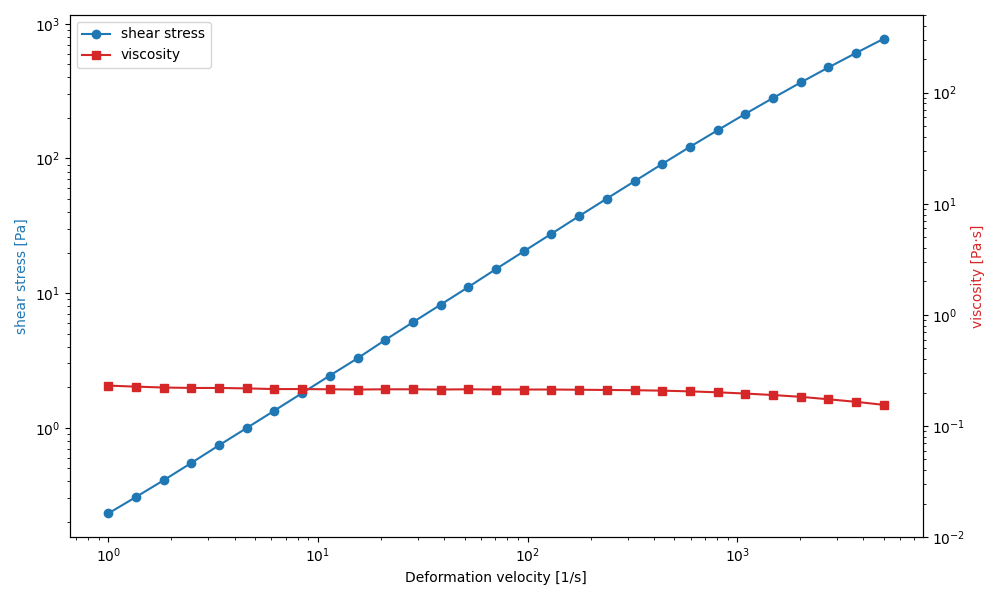
\includegraphics[scale = 0.5]{Bilder/14_PVP.png}
			\caption{The graph shows the measurements of 14\%-PVP solution. 
			On the left y-axis the shear stress and on the right y-axis the velocity is plotted, both of these are plotted against the deformation velocity.}
			\label{14PVP}
		\end{figure}

		The final measurement of this exercise was the measurement of a 50\% starch solution. Graph \ref{starch} shows a clear exponential funktion wich points to a non newtonian shear thickening fluid.
		Meaning the viscosity is increasing when increasing the deformation velocity.
		This is not that surprising because starch is also the main ingredient of oobleck and the properties are pretty known.


		\begin{figure}[H]
			\centering
			
\includegraphics[scale = 0.5]{Bilder/Speisestärke.png}
			\caption{The graph shows the measurements of a starch solution. 
			On the left y-axis the shear stress and on the right y-axis the velocity is plotted, both of these are plotted against the deformation velocity.}
			\label{starch}
		\end{figure}

	
	\subsection{Time dependant measurement of the viscosity}


		\begin{figure}[H]
			\centering
			
\includegraphics[scale = 0.75]{Bilder/ketchup.png}
			\caption{The graph shows the three time dependant viscosity measurements of ketchup. The shear viscosity is plotted against the duration.}
			\label{ketchup}
		\end{figure}


	\subsection{Oszillational measurements to determine the viscoelastic properties}

	
	\subsubsection{Amplitude sweep}

		

		\begin{figure}[H]
			\centering
			
\includegraphics[scale = 0.75]{Bilder/20_PVP_amp_eta.png}
			\caption{This graph shows the complex viscosity plotted against the deformation of 20\%-PVP solution at constant frequency.}
			\label{20_PVP_amp_eta}
		\end{figure}


		\begin{figure}[H]
			\centering
			
\includegraphics[scale = 0.75]{Bilder/20_PVP_amp_G1.png}
			\caption{This graph shows the storage module G' plotted against the deformation of 20\%-PVP solution at constant frequency.}
			\label{20_PVP_amp_G1}
		\end{figure}


		\begin{figure}[H]
			\centering
			
\includegraphics[scale = 0.75]{Bilder/20_PVP_amp_G2.png}
			\caption{This graph shows the loss module G'' plotted against the deformation of 20\%-PVP solution at constant frequency.}
			\label{20_PVP_amp_G2}
		\end{figure}

	\subsubsection{Frequency sweep}

		\begin{figure}[H]
			\centering
			
\includegraphics[scale = 0.75]{Bilder/20_PVP_frq_betragEta.png}
			\caption{This graph shows the complex viscosity plotted against the deformation of 20\%-PVP solution at constant amplitude.}
			\label{20_PVP_frq_betragEta}
		\end{figure}

		\begin{figure}[H]
			\centering
			
\includegraphics[scale = 0.5]{Bilder/20_PVP_frq_G1_G2.png}
			\caption{This graph shows the storage module G' loss module G'' plotted against the deformation of 20\%-PVP solution at constant amplitude.}
			\label{20_PVP_frq_G1_G2}
		\end{figure}


\printbibliography

\end{document}